\documentclass[tikz,border=12pt]{standalone}
\usepackage[T1]{fontenc}
\usepackage{mathpazo}
\usepackage{amsmath,amssymb}
\usetikzlibrary{arrows.meta, positioning, calc, fit, decorations.pathreplacing}

\definecolor{stblue}{HTML}{7B97AD}
\definecolor{rwgold}{HTML}{B8995E}
\definecolor{sage}{HTML}{7A9A7E}
\definecolor{dkbrown}{HTML}{3D3530}
\definecolor{wmgray}{HTML}{7B7067}
\definecolor{cream}{HTML}{F9F6F0}
\definecolor{border}{HTML}{D4C9B8}
\definecolor{terracotta}{HTML}{C47A6A}
\definecolor{lavender}{HTML}{907EA0}

\begin{document}
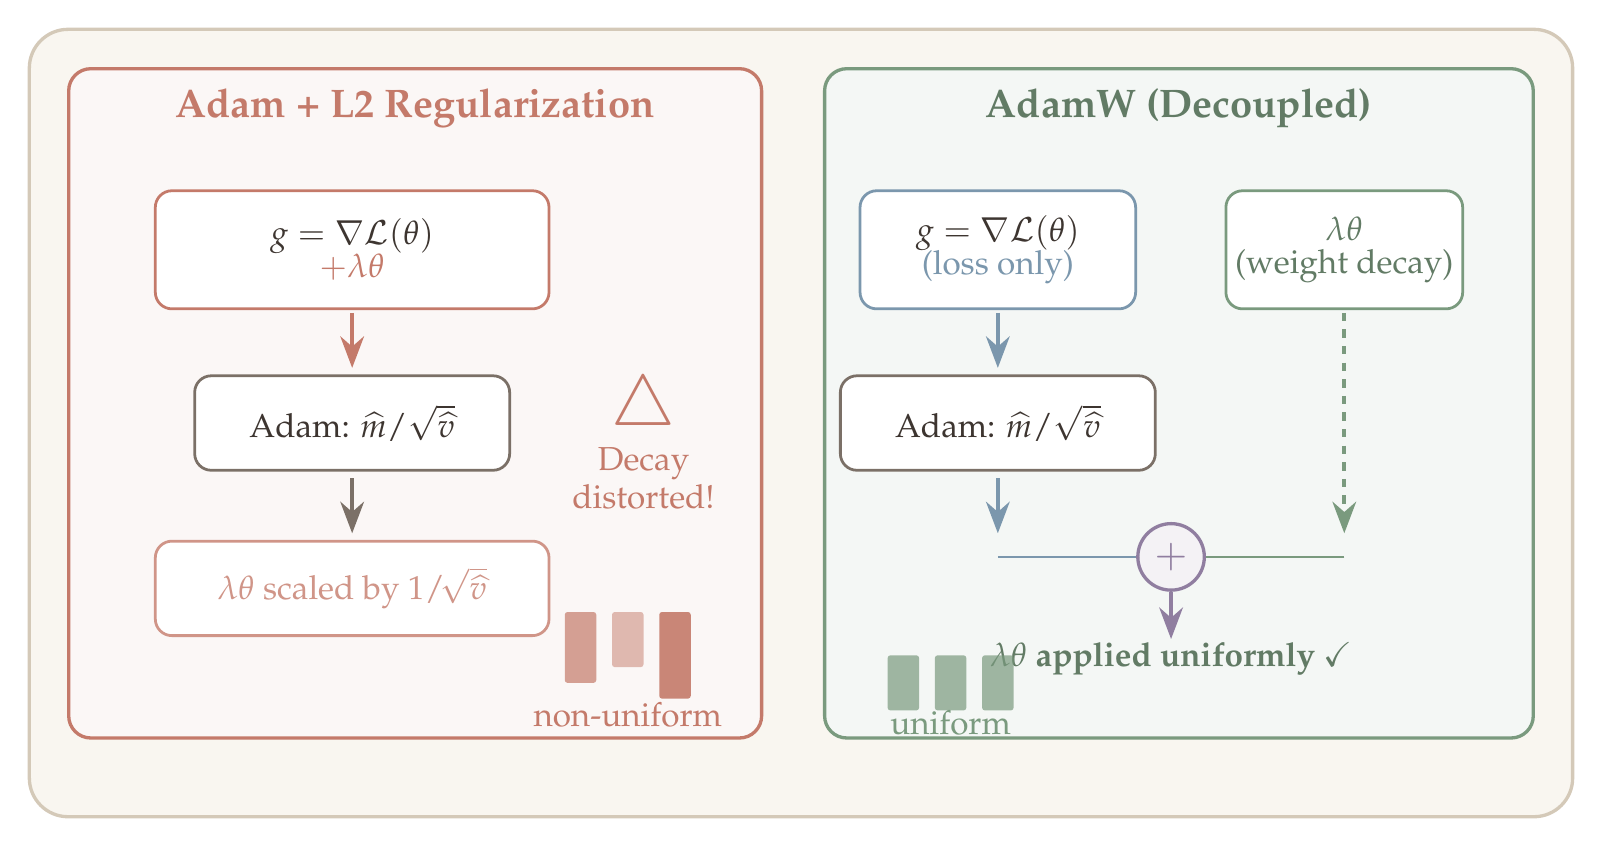
\begin{tikzpicture}[>={Stealth[length=4mm, width=3mm]}, line width=1.5pt]

% Background
\fill[cream, rounded corners=14pt] (-0.3,-1.0) rectangle (19.3,9.0);
\draw[border, line width=1.2pt, rounded corners=14pt] (-0.3,-1.0) rectangle (19.3,9.0);

%% LEFT PANEL: Adam + L2
\fill[terracotta!6, rounded corners=8pt] (0.2,0.0) rectangle (9.0,8.5);
\draw[terracotta, line width=1.2pt, rounded corners=8pt] (0.2,0.0) rectangle (9.0,8.5);
\node[text=terracotta, font=\Large\bfseries] at (4.6,8.0) {Adam + L2 Regularization};

% Gradient box (includes lambda*theta)
\node[draw=terracotta, line width=1pt, fill=white, rounded corners=6pt,
      minimum width=5.0cm, minimum height=1.5cm, align=center, text=dkbrown, font=\large]
      (gradL) at (3.8,6.2) {$g = \nabla\mathcal{L}(\theta)$\\[-2pt]
      {\color{terracotta}\textbf{$+ \lambda\theta$}}};

% Arrow down
\draw[terracotta, ->, line width=1.5pt] (3.8,5.4) -- (3.8,4.7);

% Adam processing box
\node[draw=wmgray, line width=1pt, fill=white, rounded corners=6pt,
      minimum width=4.0cm, minimum height=1.2cm, text=dkbrown, font=\large] (adamL) at (3.8,4.0)
      {Adam: $\widehat{m}/\sqrt{\widehat{v}}$};

% Arrow down
\draw[wmgray, ->, line width=1.5pt] (3.8,3.3) -- (3.8,2.6);

% Result box
\node[draw=terracotta!80, line width=1pt, fill=white, rounded corners=6pt,
      minimum width=5.0cm, minimum height=1.2cm, text=terracotta!80, align=center, font=\large]
      (resultL) at (3.8,1.9) {$\lambda\theta$ scaled by $1/\!\sqrt{\widehat{v}}$};

% Warning annotation
\node[text=terracotta, font=\Huge] at (7.5,4.2) {$\triangle$};
\node[text=terracotta, font=\large, align=center] at (7.5,3.3) {Decay\\distorted!};

% Non-uniform bars
\fill[terracotta, opacity=0.7, rounded corners=1pt] (6.5,0.7) rectangle (6.9,1.6);
\fill[terracotta, opacity=0.5, rounded corners=1pt] (7.1,0.9) rectangle (7.5,1.6);
\fill[terracotta, opacity=0.9, rounded corners=1pt] (7.7,0.5) rectangle (8.1,1.6);
\node[text=terracotta, font=\large] at (7.3,0.3) {non-uniform};

%% RIGHT PANEL: AdamW
\fill[sage!8, rounded corners=8pt] (9.8,0.0) rectangle (18.8,8.5);
\draw[sage, line width=1.2pt, rounded corners=8pt] (9.8,0.0) rectangle (18.8,8.5);
\node[text=sage!80!black, font=\Large\bfseries] at (14.3,8.0) {AdamW (Decoupled)};

% Gradient box (loss only)
\node[draw=stblue, line width=1pt, fill=white, rounded corners=6pt,
      minimum width=3.5cm, minimum height=1.5cm, align=center, text=dkbrown, font=\large]
      (gradR) at (12.0,6.2) {$g = \nabla\mathcal{L}(\theta)$\\[-2pt]
      {\color{stblue}\large(loss only)}};

% Weight decay box (separate)
\node[draw=sage, line width=1pt, fill=white, rounded corners=6pt,
      minimum width=3.0cm, minimum height=1.5cm, align=center, text=sage!80!black, font=\large]
      (wdR) at (16.4,6.2) {$\lambda\theta$\\[-2pt]
      {\large(weight decay)}};

% Arrow: gradient through Adam
\draw[stblue, ->, line width=1.5pt] (12.0,5.4) -- (12.0,4.7);

% Adam processing box
\node[draw=wmgray, line width=1pt, fill=white, rounded corners=6pt,
      minimum width=4.0cm, minimum height=1.2cm, text=dkbrown, font=\large] (adamR) at (12.0,4.0)
      {Adam: $\widehat{m}/\sqrt{\widehat{v}}$};

% Arrow: Adam output down
\draw[stblue, ->, line width=1.5pt] (12.0,3.3) -- (12.0,2.6);

% Arrow: weight decay goes straight down (bypassing Adam)
\draw[sage, ->, line width=1.5pt, dashed] (16.4,5.4) -- (16.4,2.6);

% Combine circle
\node[draw=lavender, line width=1.2pt, fill=lavender!10, circle,
      inner sep=3pt, font=\Large\bfseries, text=lavender] (mergeR) at (14.2,2.3) {$+$};

% Lines to combine circle
\draw[stblue, line width=1pt] (12.0,2.3) -- (mergeR.west);
\draw[sage, line width=1pt] (16.4,2.3) -- (mergeR.east);

% Result arrow
\draw[lavender, ->, line width=1.5pt] (mergeR.south) -- ++(0,-0.6);
\node[text=sage!80!black, font=\large\bfseries] at (14.2,1.0) {$\lambda\theta$ applied uniformly \checkmark};

% Uniform bars
\fill[sage, opacity=0.7, rounded corners=1pt] (10.6,0.35) rectangle (11.0,1.05);
\fill[sage, opacity=0.7, rounded corners=1pt] (11.2,0.35) rectangle (11.6,1.05);
\fill[sage, opacity=0.7, rounded corners=1pt] (11.8,0.35) rectangle (12.2,1.05);
\node[text=sage, font=\large] at (11.4,0.2) {uniform};

\end{tikzpicture}
\end{document}
